\indent\indent The \textit{Disp. vs Pos.} feature from the \textit{Masks} menu helps you to compare the displacement of each marker depending on its position in the X or Y direction. Select the markers that you would like to hide and confirm to apply the mask on your data.\\
\newline
\indent This tool gives you a fast and easy way to detect wrong behaviour in your markers. All markers will in most of the case follow a certain trend in one direction and you can then locate markers with correlation issues.\\

\begin{figure}[!h]
   \centering
   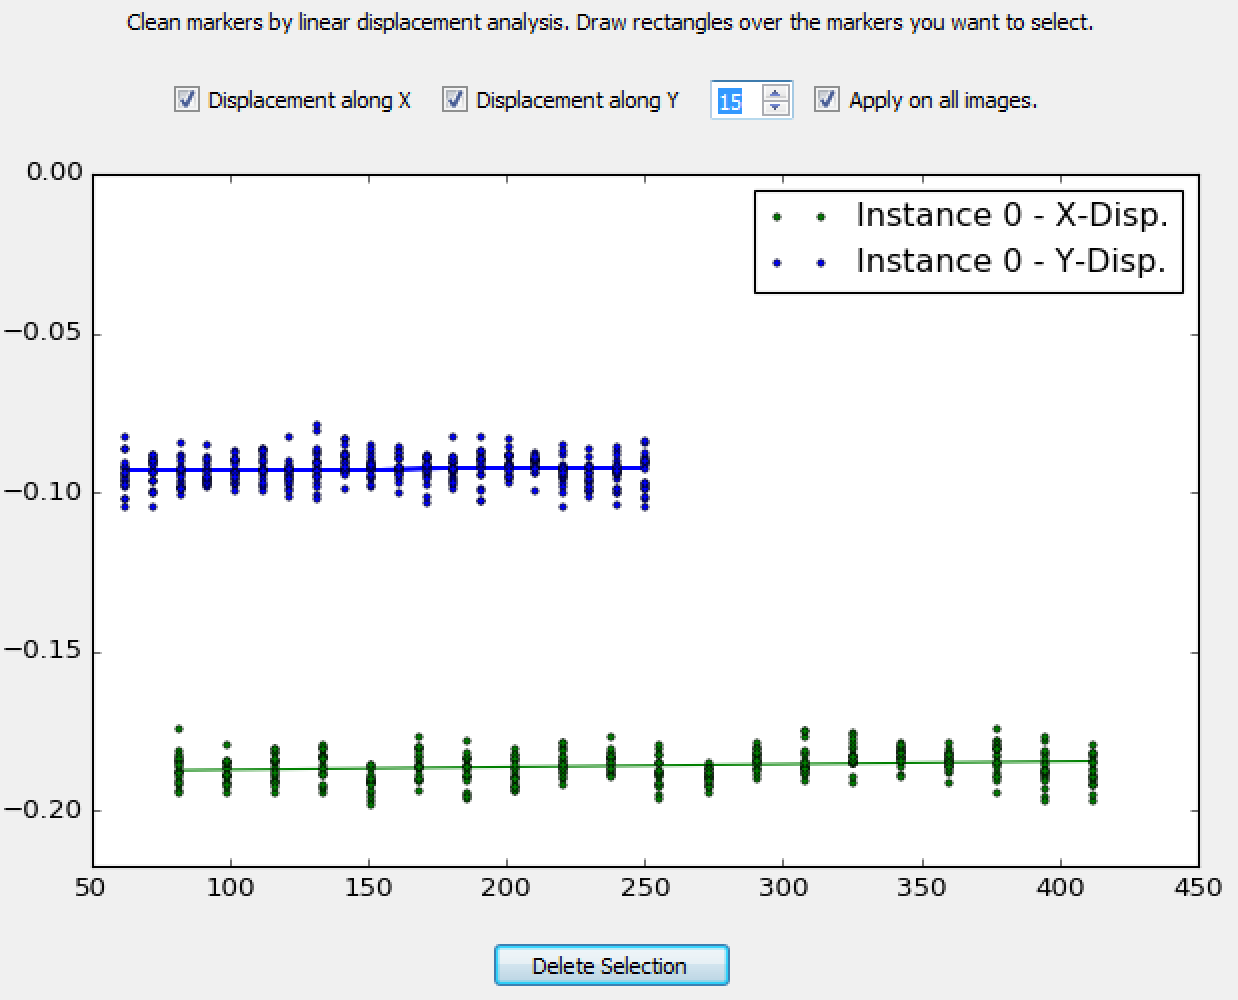
\includegraphics[scale=.4]{disp_vs_pos}
   \caption{Disp. vs Pos. - Hide markers with wrong behaviour}
\end{figure}

\newline
\indent When a mask is applied, the previous state of the analysis is automatically saved in the analysis folder.\\
On start-up, the software will load the last mask version by default. If you made a mistake or want to bring back your data, you can open a previous version by using the \text{Open Mask/Version} option in the \textit{File} menu.\\
\newline
\indent Please keep in mind that when a mask is applied, the data is only hidden and not modified. An older version can always be loaded.
